\documentclass[12pt,a4paper]{article}

% ---------- Pacotes ----------
% Fontes
\usepackage{fontspec}
\setmainfont{Aptos.ttf}[
    BoldFont = Aptos-Bold.ttf,
    ItalicFont = Aptos-Italic.ttf,
    BoldItalicFont = Aptos-Italic.ttf
]

% Para usar fontes diferentes:
\usepackage{anyfontsize}

% Retira espaço extra obsoleto entre as frases.
\frenchspacing

% Para identar primeiro parágrafo:
\usepackage{indentfirst}

% Para customizar as margens:
\usepackage[left=3.175cm,right=3.175cm,top=2.54cm,bottom=3.0cm]{geometry}

% Para customizar os gráficos:
\usepackage{float}
\usepackage{graphicx}

% Para customizar as cores:
\usepackage{xcolor}
\definecolor{codebg}{RGB}{245,245,245}
\definecolor{codeframe}{RGB}{200,200,200}
\definecolor{trad-blue}{RGB}{31,74,145}
\definecolor{cover-rule}{RGB}{68,114,196}

% Para customizar os links:
\usepackage{hyperref}
% Para trocar o estilo dos hyperlinks:
\hypersetup{
  colorlinks   = true, % Colours links instead of ugly boxes
  urlcolor     = blue, % Colour for external hyperlinks
  linkcolor    = blue, % Colour of internal links
  citecolor    = blue, % Colour of citations
  linktocpage  = true, % Link only on page numbers
}

% Para acrescentar comentários ao PDF descomente:
\hypersetup{
  pdftitle     = {Módulo I: Git - Atividade prática},
  pdfauthor    = {João V. S. Guerra},
  pdfkeywords  = {git, TRAD2026, tutorial, LNBio, LNBR, CNPEM},
  pdfproducer  = {Latex with hyperref},
  pdfcreator   = {pdflatex}
}

% Para usar letras no enumerate:
\usepackage{enumitem}
\setlist[enumerate,1]{leftmargin=1.6em}

% Para usar símbolos matemáticos:
\usepackage{amssymb}

% Para customizar o cabeçalho e rodapé:
\usepackage{fancyhdr}
\usepackage{lastpage}

% Para colocar imagens de fundo:
\usepackage{eso-pic}

% Para customizar os blocos de código:
\usepackage{listings}
\lstdefinestyle{shell}{
    backgroundcolor=\color{codebg},
    basicstyle=\ttfamily\small,
    frame=single,
    rulecolor=\color{codeframe},
    breaklines=true,
    breakatwhitespace=false,
    columns=fullflexible,
    keepspaces=true,
    xleftmargin=1em,
    xrightmargin=1em,
    framexleftmargin=0.8em,
    framexrightmargin=0.8em,
    aboveskip=8pt,
    belowskip=8pt,
    showstringspaces=false,
}
\lstset{style=shell}

% Header
\AddToShipoutPictureBG{%
  \AtPageUpperLeft{%
    \raisebox{-\height}{
\includegraphics[width=\paperwidth]{images/header.png}}%
  }%
}

% Footer
\AddToShipoutPictureBG{%
  \AtPageLowerLeft{%
    
\includegraphics[width=\paperwidth]{images/footer.png}%
  }%
}

% Para customizar os blocos de perguntas:
\usepackage[most]{tcolorbox}
\newtcolorbox{question}[1]{   % [1] means it takes 1 argument
    enhanced,
    colback=white,
    colframe=trad-blue,
    colback=cover-rule!10,
    attach boxed title to top left={yshift*=-\tcboxedtitleheight}, 
    title=\texttt{#1},        % use the argument as the title
    boxed title size=title,
    boxed title style={%
        rounded corners=northeast, 
        rounded corners=northwest, 
        colback=tcbcolframe, 
        boxrule=0pt,
    },
    underlay boxed title={%
        \path[fill=tcbcolframe] (title.south west)--(title.south east) 
            to[out=0, in=180] ([xshift=5mm]title.east)--
            (title.center-|frame.east)
            [rounded corners=5pt] |- 
            (frame.north) -| cycle; 
    },
}

% Para customizar o sumário:
\renewcommand{\contentsname}{\centering Sumário}

% Para colocar o número da página dentro do círculo azul no rodapé:
\usepackage{tikz}
% Define the custom circled page number
\newcommand{\bluecirclepage}{%
  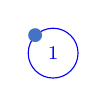
\begin{tikzpicture}[baseline=(char.base)]
    \node[shape=circle, draw=blue, text=blue, inner sep=2pt, minimum size=18pt] (char) {\scriptsize\thepage};
    \fill[cover-rule] (char.135) circle (2.5pt);
  \end{tikzpicture}%
}
\pagestyle{fancy}
\fancyhf{}
\fancyfootoffset[R]{2.5cm}
\rfoot{\raisebox{10pt}{\bluecirclepage}}
\renewcommand{\headrulewidth}{0pt}

% Para customizar o espaçamento entre linhas:
\usepackage{setspace}

\begin{document}

% ---------- Cabeçalho ----------
\begin{center}
    \vspace*{0.2cm}
    \makebox[\linewidth][c]{
\includegraphics[width=1.2\textwidth]{images/logo.png}}


    \vspace{7.5em}
    {\color{cover-rule}\rule{\textwidth}{2.25pt}}

    \vspace{1em}
    {\fontsize{48}{48}\selectfont \textbf{Módulo I: Git}}

    \vspace{2em}
    {\fontsize{20}{20}\selectfont \emph{Atividade prática}}

    \vspace{2em}
    {\color{cover-rule}\rule{\textwidth}{2.25pt}}
    \vspace{13em}

    \begin{center}
        
\includegraphics[width=0.20\textwidth]{images/lnbio.png}\hspace{1em}%
        
\includegraphics[width=0.22\textwidth]{images/lnbr.png}
    \end{center}
\end{center}

\thispagestyle{empty}

\clearpage

\setstretch{1.5}
\setlength{\parindent}{0pt}
\setlength{\parskip}{6pt}

\tableofcontents

\clearpage

\section{Comandos git na prática}

Nesta atividade, você irá explorar os principais comandos do Git, aplicando-os em um repositório local. Siga as instruções abaixo para completar a atividade.

\subsection{Configuração inicial}

Antes de começar a usar o Git, é importante configurar seu nome e endereço de e-mail. Essas informações serão associadas aos commits e ajudarão a identificar suas contribuições no repositório. 

\begin{lstlisting}[language=bash]
git config --global user.name "Seu Nome"
git config --global user.email "seu.email@example.com" 
\end{lstlisting}

\begin{question}{Dica.}
Se você for colaborar em um projeto com outros desenvolvedores, é recomendável usar o mesmo nome e email que você utiliza no GitHub ou em outras plataformas de hospedagem de código.
\end{question}

Por padrão, o git cria o branch principal com o nome \textbf{\texttt{master}}. No entanto, é uma boa prática utilizar o nome \textbf{\texttt{main}} para o branch principal. Para configurar isso, use o comando abaixo:


\end{document}
